% Template of basic phisics experiment 基于 article template, 在此基础上做修改
% 设定文章编码类型, 正文字号为五号则 zihao=5, 正文字号为小四则 zihao=-4
\documentclass[zihao=5, UTF8]{article}		


% 自定义宏定义
\def\N{\mathbb{N}}
\def\F{\mathbb{F}}
\def\Z{\mathbb{Z}}
\def\Q{\mathbb{Q}}
\def\R{\mathbb{R}}
\def\C{\mathbb{C}}
\def\T{\mathbb{T}}
\def\S{\mathbb{S}}
\def\A{\mathbb{A}}
\def\I{\mathscr{I}}
\def\d{\mathrm{d}}
\def\p{\partial}


% 物理实验报告所需的其它宏包
\usepackage{ulem}   % \uline 下划线支持

% 导入基本宏包
\usepackage[UTF8]{ctex}     % 设置文档为中文语言
\usepackage[colorlinks, linkcolor=blue, anchorcolor=blue, citecolor=blue, urlcolor=blue]{hyperref}  % 宏包：自动生成超链接 (此宏包与标题中的数学环境冲突)
% \usepackage{docmute}    % 宏包：子文件导入时自动去除导言区, 用于主/子文件的写作方式, \include{./51单片机笔记}即可. 注：启用此宏包会导致.tex文件capacity受限. 
\usepackage{amsmath}    % 宏包：数学公式
\usepackage{bm}
\usepackage{mathrsfs}   % 宏包：提供更多数学符号
\usepackage{amssymb}    % 宏包：提供更多数学符号
\usepackage{pifont}     % 宏包：提供了特殊符号和字体
\usepackage{extarrows}  % 宏包：更多箭头符号
\usepackage{multirow}

% 列表环境设置
\usepackage{enumitem}   % 宏包：列表环境设置
    \setlist[enumerate]{itemsep=0pt, parsep=0pt, topsep=0pt, partopsep=0pt, leftmargin=3.5em} 
    \setlist[itemize]{itemsep=0pt, parsep=0pt, topsep=0pt, partopsep=0pt, leftmargin=3.5em}
    \newlist{circledenum}{enumerate}{1} % 创建一个新的枚举环境  
    \setlist[circledenum,1]{  
        label=\protect\circled{\arabic*}, % 使用 \arabic* 来获取当前枚举计数器的值, 并用 \circled 包装它  
        ref=\arabic*, % 如果需要引用列表项, 这将决定引用格式（这里仍然使用数字）
        itemsep=0pt, parsep=0pt, topsep=0pt, partopsep=0pt, leftmargin=3.5em
    }  
% 文章页面 margin 设置
\usepackage[a4paper]{geometry}  % 宏包：文章页面 margin 设置
    \geometry{top=0.75in}
    \geometry{bottom=0.75in}
    \geometry{left=0.75in}
    \geometry{right=0.75in}   % 设置上下左右页边距
    \geometry{marginparwidth=1.75cm}    % 设置边注距离（注释、标记等）

% 自定义数学环境
\usepackage{amsthm} % 宏包：数学环境配置
% theorem-line 环境自定义
    \newtheoremstyle{MyLineTheoremStyle}% <name>
        {11pt}% <space above>
        {11pt}% <space below>
        {}% <body font> 使用默认正文字体
        {}% <indent amount>
        {\bfseries}% <theorem head font> 设置标题项为加粗
        {：}% <punctuation after theorem head>
        {.5em}% <space after theorem head>
        {\textbf{#1}\thmnumber{#2}\ \ (\,\textbf{#3}\,)}% 设置标题内容顺序
    \theoremstyle{MyLineTheoremStyle} % 应用自定义的定理样式
    \newtheorem{LineTheorem}{Theorem.\,}
% theorem-block 环境自定义
    \newtheoremstyle{MyBlockTheoremStyle}% <name>
        {11pt}% <space above>
        {11pt}% <space below>
        {}% <body font> 使用默认正文字体
        {}% <indent amount>
        {\bfseries}% <theorem head font> 设置标题项为加粗
        {：\\ \indent}% <punctuation after theorem head>
        {.5em}% <space after theorem head>
        {\textbf{#1}\thmnumber{#2}\ \ (\,\textbf{#3}\,)}% 设置标题内容顺序
    \theoremstyle{MyBlockTheoremStyle} % 应用自定义的定理样式
    \newtheorem{BlockTheorem}[LineTheorem]{Theorem.\,} % 使用 LineTheorem 的计数器
% definition 环境自定义
    \newtheoremstyle{MySubsubsectionStyle}% <name>
        {11pt}% <space above>
        {11pt}% <space below>
        {}% <body font> 使用默认正文字体
        {}% <indent amount>
        {\bfseries}% <theorem head font> 设置标题项为加粗
        {：\\ \indent}% <punctuation after theorem head>
        {0pt}% <space after theorem head>
        {\textbf{#3}}% 设置标题内容顺序
    \theoremstyle{MySubsubsectionStyle} % 应用自定义的定理样式
    \newtheorem{definition}{}


% 有色文本框及其设置
\usepackage[dvipsnames,svgnames]{xcolor}    %设置插入的文本框颜色
\usepackage[strict]{changepage}     % 提供一个 adjustwidth 环境
\usepackage{framed}     % 实现方框效果
    \definecolor{graybox_color}{rgb}{0.95,0.95,0.96} % 文本框颜色. 修改此行中的 rgb 数值即可改变方框纹颜色, 具体颜色的rgb数值可以在网站https://colordrop.io/ 中获得. （截止目前的尝试还没有成功过, 感觉单位不一样）（找到喜欢的颜色, 点击下方的小眼睛, 找到rgb值, 复制修改即可）
    \newenvironment{graybox}{%
    \def\FrameCommand{%
    \hspace{1pt}%
    {\color{gray}\small \vrule width 2pt}%
    {\color{graybox_color}\vrule width 4pt}%
    \colorbox{graybox_color}%
    }%
    \MakeFramed{\advance\hsize-\width\FrameRestore}%
    \noindent\hspace{-4.55pt}% disable indenting first paragraph
    \begin{adjustwidth}{}{7pt}%
    \vspace{2pt}\vspace{2pt}%
    }
    {%
    \vspace{2pt}\end{adjustwidth}\endMakeFramed%
    }

% 各级标题自定义设置
\usepackage{titlesec}   
    % section标题自定义设置 
    \titleformat{\section}[hang]{\normalfont\huge\bfseries\centering}{第\,\thesection\,部分}{20pt}{}
    % subsection标题自定义设置 
    \titleformat{\subsection}[hang]{\normalfont\Large\bfseries}{\,\thesubsection\,}{8pt}{}
    % subsubsection标题自定义设置
    \titleformat{\subsubsection}[hang]{\normalfont\large\bfseries}{\,\thesubsubsection\,}{6pt}{}

% 外源代码插入设置
\usepackage{matlab-prettifier}
    \lstset{
        style=Matlab-editor,  % 继承matlab代码颜色等
    }
\usepackage[most]{tcolorbox} % 引入tcolorbox包 
\usepackage{listings} % 引入listings包
    \tcbuselibrary{listings, skins, breakable}
    \lstdefinestyle{matlabstyle}{
        language=Matlab,
        basicstyle=\small,
        breakatwhitespace=false,
        breaklines=true,
        captionpos=b,
        keepspaces=true,
        numbers=left,
        numbersep=15pt,
        showspaces=false,
        showstringspaces=false,
        showtabs=false,
        tabsize=2
    }
    \newtcblisting{matlablisting}{
        arc=0pt,
        top=0pt,
        bottom=0pt,
        left=1mm,
        listing only,
        listing style=matlabstyle,
        breakable,
        colback=white   % 选一个合适的颜色
    }

% table 支持
\usepackage{booktabs}   % 宏包：三线表
\usepackage{tabularray} % 宏包：表格排版
\usepackage{longtable}  % 宏包：长表格

% figure 设置
\usepackage{graphicx}  % 支持 jpg, png, eps, pdf 图片 
\usepackage{svg}       % 支持 svg 图片
    \svgsetup{
        % 指向 inkscape.exe 的路径
        inkscapeexe = C:/aa_MySame/inkscape/bin/inkscape.exe, 
        % 一定程度上修复导入后图片文字溢出几何图形的问题
        inkscapelatex = false                 
    }


% 图表进阶设置
\usepackage{float}     % 图表位置浮动设置 
\usepackage{caption}    % 图注、表注
    \captionsetup[figure]{name=图}  
    \captionsetup[table]{name=表}
    \captionsetup{labelfont=bf, font=small}

%% 文章默认字体设置
%    \usepackage{fontspec}   % 宏包：字体设置
%        \setmainfont{SimSun}[
%            BoldFont = SimHei, % 设置粗体字为黑体
%            ItalicFont = KaiTi, % 设置斜体字为楷体
%            BoldItalicFont = KaiTi % 设置粗斜体字为楷体
%        ] 
%        %\setCJKmainfont[AutoFakeBold=3]{SimSun} % 设置加粗字体为 SimSun 族, AutoFakeBold 可以调整字体粗细
%        \setmainfont{Times New Roman} % 设置英文字体为Times New Roman


% 其它设置
    % equation 公式编号设置
        \makeatletter  
        \renewcommand{\theequation}{\thesection.\arabic{equation}}  
        \makeatother
    % 脚注设置
        \renewcommand\thefootnote{\ding{\numexpr171+\value{footnote}}}
    % 参考文献引用设置
        \bibliographystyle{unsrt}   % 设置参考文献引用格式为unsrt
        \newcommand{\upcite}[1]{\textsuperscript{\cite{#1}}}     % 自定义上角标式引用
    % 文章序言设置
        \newcommand{\cnabstractname}{序言}
        \newenvironment{cnabstract}{%
            \par\Large
            \noindent\mbox{}\hfill{\bfseries \cnabstractname}\hfill\mbox{}\par
            \vskip 2.5ex
            }{\par\vskip 2.5ex}


% 页眉页脚设置
\usepackage{fancyhdr}   %宏包：页眉页脚设置
    \pagestyle{fancy}
    \fancyhf{}
    \cfoot{\thepage}
    \renewcommand\headrulewidth{1pt}
    \renewcommand\footrulewidth{0pt}
    \rhead{\bfseries 分组序号: 3-04-1}    
    \chead{《基础物理实验》实验报告,\ 潘天麟\ 2023K8009908023}
    \lhead{2024.11.13}

\usepackage{pdfpages}

% 开始编辑文章

\begin{document}
\noindent\begin{flushright}
    \zihao{2}{分组序号: 3-04-1}
\end{flushright}

\newcommand*{\boldsong}{\CJKfamily{boldsong}}


\begin{center}\large
    \noindent{\Huge\bfseries\boldsong《基础物理实验》实验报告 }
    \\\vspace{0.4cm}
    \noindent\textit{
        \textbf{\boldsong 实验名称：}\uline{\hspace{2.3cm} 驻波实验\hspace{2.3cm}}\hspace{0.4cm} 
        指导教师：\uline{\hspace{1.5cm}杨俊亮\hspace{1.5cm}}}
    \\\vspace{0.1cm}
    \noindent\textit{
        姓名：\uline{\,\,潘天麟\,\,}\hspace{0.2cm}
        学号：\uline{\,\,{\upshape 2023K8009908023}\,\,}\hspace{0.2cm}
        专业：\uline{\,\,人工智能\,\,}\hspace{0.2cm}
        班级：\uline{\,\,\upshape{2313}\,\,}\,组号：\uline{\,\,\upshape{3-04-1}\,\,}}
    \\\vspace{0.1cm}
    \noindent\textit{
        实验日期：\uline{\,\,{\upshape 2024.11.13}\,\,}\hspace{0.2cm}
        实验地点：\uline{\,\,\,教学楼{\upshape721}\,\,\,}\hspace{0.2cm}
        是否调课/补课：\uline{\,\,否\,\,}\hspace{0.2cm}
        成绩：\uline{\hspace{2cm}}}
\end{center}
% \vspace{-0.2cm}
\noindent\rule{\textwidth}{0.1em}   % 分割线

% 控制目录不换页
\vspace{1cm}
\setcounter{tocdepth}{3}  % 目录深度为 2（不显示 subsubsection）
\noindent\begin{minipage}{\textwidth}\centering
\tableofcontents\thispagestyle{fancy}   % 显示页码、页眉等   
\end{minipage}  
\newpage

\section{弦上驻波实验}
\subsection{实验目的}
\begin{enumerate}
    \item 了解弦线达到共振和形成稳定驻波的条件;
    \item 观察在两端固定的弦线上形成的驻波现象;
    \item 测定弦线上横波的传播速度;
    \item 用实验的方法确定弦线作受迫振动时共振频率$f$与半波长个数$n$、弦线有效长度$l$、张力$T$及弦密度$\mu$之间的关系;
    \item 用对数作图和最小乘法对共振频率与张力关系的实验结果作线性拟合, 处理数据, 并给出结论. 
\end{enumerate}
\subsection{实验仪器}
\begin{enumerate}
    \item 弦音仪（弦乐器的模拟装置）
    \item 信号发生器
    \item 双踪示波器
    \item 电子天平
    \item 精密电子天平
    \item 钢尺
    \item 螺旋测微仪
    \item 500g标准砝码
\end{enumerate}
\subsection{实验原理}
\subsubsection{弦上驻波产生的原理}

当弦长$L$与波长$\lambda$之间的关系可以使得前进波和许多反射波都有相同的相位时, 弦线上的各点都做各自恒定的简谐振动. 则弦线上有些点振动的振幅最大, 称为波腹;而另外有些点的振幅为零, 称为波节, 这就形成了\textbf{驻波}现象.

\subsubsection{数学推导}
相邻两波节/波腹间距为半波长, 而弦线两端固定, 即两端都是波节, 则弦线长度 $L$ 应为半波长整数倍. 

波长 $\lambda$ 满足：
\begin{equation}
\lambda = \frac{2L}{n}, \quad n = 1,2,3,\cdots
\end{equation}

若振动频率为 $f$, 横波沿弦线传播速度为
\begin{equation}
v = \lambda f
\end{equation}

根据波动理论, 张力为 $T$, 线密度为 $\mu$, 则横波满足：
\begin{equation}
\frac{\partial^{2}y}{\partial t^{2}} = \frac{T}{\mu}\frac{\partial^{2}y}{\partial x^{2}}
\end{equation}

或等价地, 
\begin{equation}
\frac{\partial^{2}y}{\partial t^{2}} = v^{2}\frac{\partial^{2}y}{\partial x^{2}}
\end{equation}

式中 $x$ 为波在传播方向（与弦线平行）的位置坐标, $y$ 为振动位移. 

通过比较得到波的传播速度
\begin{equation}
v = \sqrt{\frac{T}{\mu}}
\end{equation}

又由于 $v = \lambda f$, 得
\begin{equation}
\lambda = \frac{1}{f}\sqrt{\frac{T}{\mu}}
\end{equation}

两边取对数
\begin{equation}
\log\lambda = \frac{1}{2}\log T - \frac{1}{2}\log\mu - \log f
\end{equation}

根据公式, 若固定 $f$ 及 $\mu$, 改变张力 $T$, 测出各相应波长 $\lambda$, 作 $\log \lambda - \log T$ 图, 若得一直线, 计算其斜率值, 如为 $1/2$, 则证明了 $\lambda \propto {T}^{1/2}$ 的关系成立. 同理, 固定线密度 $\mu$ 及 $T$ 改变振动频率 $f$, 测出各相应波长 $\lambda$, 作 $\log \lambda - \log f$ 图, 如得到斜率为 $-1$ 的直线则验证了 $\lambda \propto {f}^{-1}$. 

弦线上的波长可利用驻波原理测量. 当两个振幅和频率相同的相干波在同一直线上相向传播时, 其所叠加而成的波称为驻波, 一维驻波是波干涉中的一种特殊情形. 在弦线上出现许多静止点, 称为驻波的波节, 相邻两波节间的距离为半个波长. 
\subsection{实验内容}
\subsubsection{仪器的调节}
\begin{enumerate}
    \item 熟悉信号发生器和弦音仪的基本构造, 在实验前注意检查仪器是否有问题, 检查完毕后, 熟悉其对应的基本功能;
    \item 将信号发生器的一个端口和示波器的一个通道相连接, 并将探测线圈连接到另一个通道上. 
\end{enumerate}

\subsubsection{测定弦的线密度}
\begin{enumerate}
    \item 检查抽屉中的弦样品和实验仪器中已经接好的弦材料是否一致, 确认材料一致后, 开始正式测量;
    \item 用标准千克砝码校准精密电子天平, 并用其测量8号弦线样品的质量;
    \item 用15cm长度的钢尺测量8号弦线样本的长度;
    \item 用螺旋测微器测量8号弦线样本的直径;
    \item 代入公式, 计算得出8号弦线样本的线密度 $\mu = \frac{m}{L}$. 
\end{enumerate}

\subsubsection{测定弦线上横波的传播速度}
\begin{enumerate}
    \item 用标准千克砝码对电子天平进行调零, 而后测出钩码的质量$m$;
    \item 将两个琴码分别放在150mm和650mm处, 用于控制弦线的有效长度为500mm;
    \item 将钩码置于第二个挂点位置, 调节仪器左下角的旋钮并观察气泡至水平状态;
    \item 调整信号发生器的输出频率, 使得弦线上形成一个稳定波腹, 记录此时弦线的振动频率$f_{1}$, 即基频;
    \item 调整信号发生器的输出频率, 使得弦线上分别形成两个和三个稳定波腹, 记录对应时刻弦线的振动频率$f_{2}$和$f_{3}$, 即二倍频和三倍频, 并拍照作记录;
    \item 再将钩码分别置于第三个和第四个挂点位置, 并重复前面(3)\textasciitilde(5)的步骤, 测出相应的数据;
    \item 根据公式$v = \sqrt{\frac{T}{\mu}}$和$T = \frac{1}{2}nmg$（$n$表示钩码在第$n$格）计算相应波速的理论值;
    \item 根据公式$v = f\lambda$和测量的数据, 计算相应波速的测量值, 其中$f$取频率的平均值;
    \item 对比分析理论值与测量值的区别, 并计算相对误差. 
\end{enumerate}

\subsubsection{探究频率和有效长度的关系}
\begin{enumerate}
    \item 固定钩码在第二个格子, 即固定$T = \frac{1}{2}\times2mg = mg$, 并调节仪器至水平;
    \item 移动两个琴码, 使得其间的有效长度$L$分别为640mm, 480mm, 320mm, 240mm, 160mm;
    \item 调整信号发生器的输出频率, 使得弦线上形成一个稳定波腹, 记录弦线在不同有效长度时对应的振动频率$f_{1}$, 即基频;
    \item 根据测得的数据计算相应的波速$v$, 从而分析得出频率$f$和有效长度$L$的关系. 
\end{enumerate}

\subsubsection{探究频率与弦线所受张力的关系}
\begin{enumerate}
    \item 移动琴码, 并固定弦线的有效长度为400mm;
    \item 分别将钩码放在不同位点处, 调节仪器至水平, 并计算对应的弦线张力$T$;
    \item 调整信号发生器的输出频率, 使得弦线上形成一个稳定波腹, 记录弦线在承受不同张力时对应的振动频率$f_{1}$, 即基频;
    \item 利用作图软件, 绘制出$\log f - \log T$曲线, 并进行线性拟合, 对比分析斜率和截距的拟合值与理论值. 
\end{enumerate}

\subsubsection{探究频率与线密度的关系}
\begin{enumerate}
    \item 共享同组人员不同号弦线的线密度$\mu$和上一实验中, 记录钩码位于第3格时候的振动频率$f_1$（基频）;
    \item 利用作图软件, 绘制出$\log f - \log \mu$曲线, 并进行线性拟合, 对比分析斜率和截距的拟合值与理论值. 
\end{enumerate}

\begin{figure}[H]
    \centering
    \begin{minipage}[t]{0.45\textwidth}
        \centering
        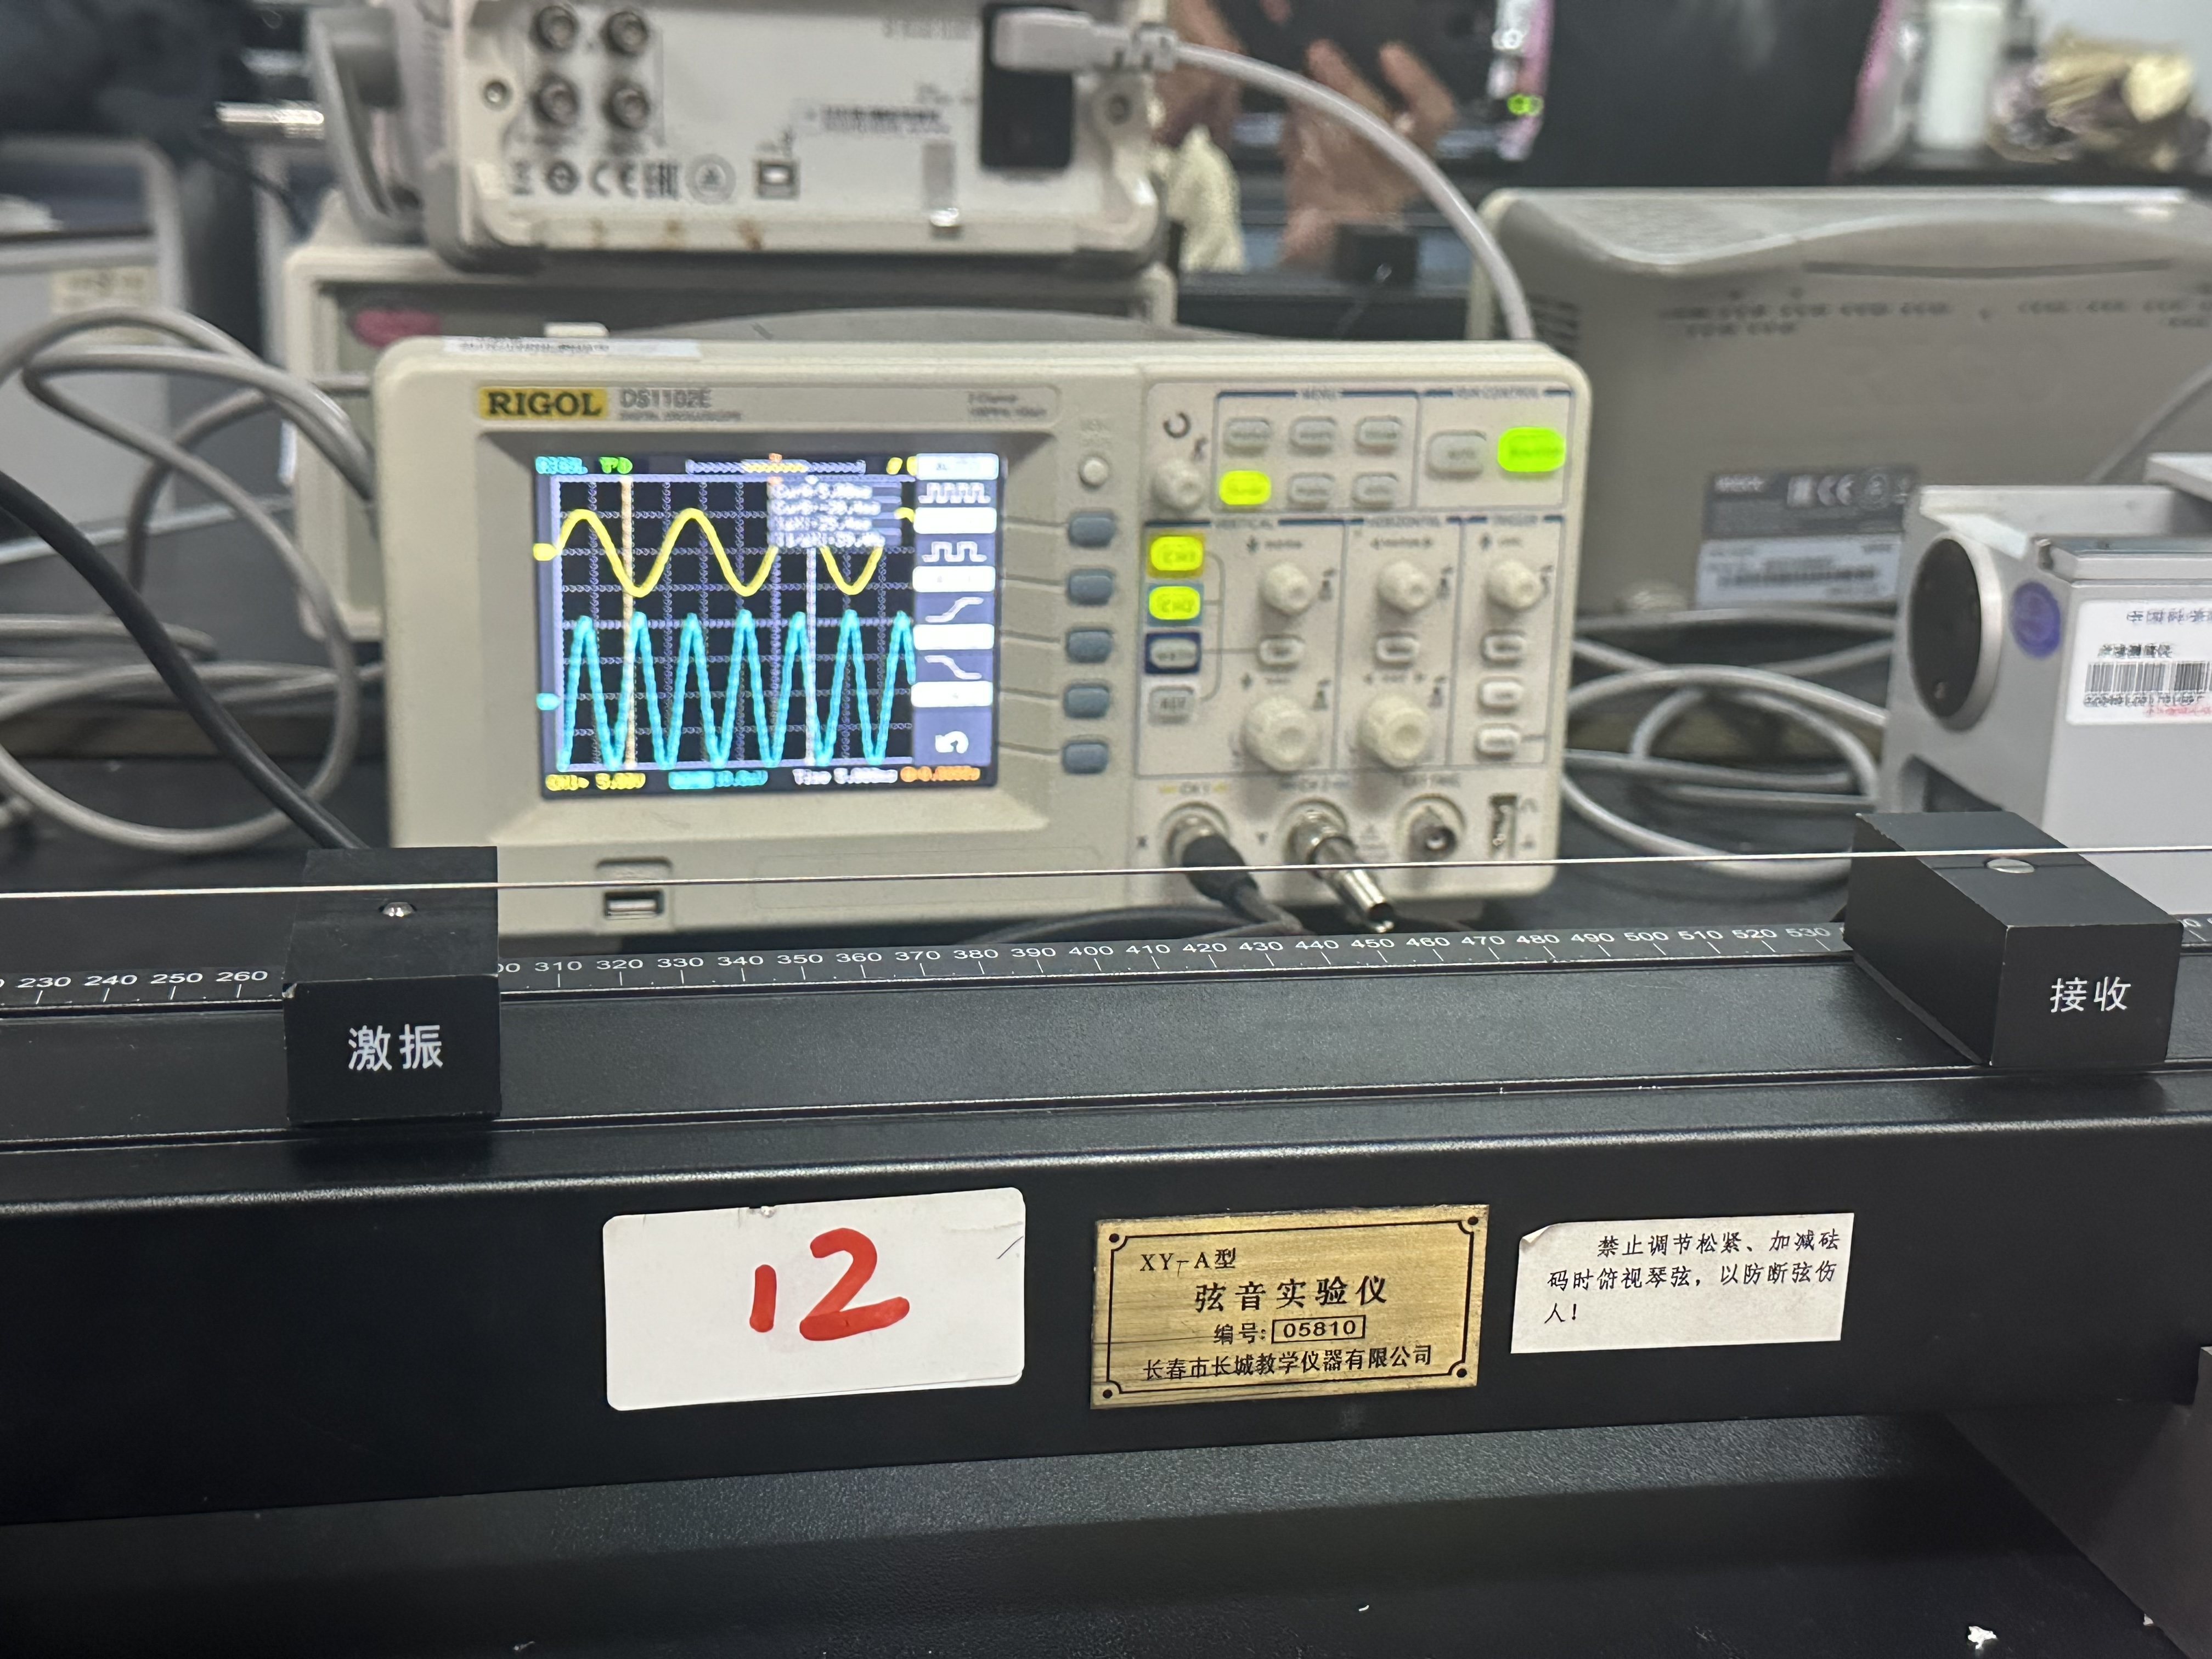
\includegraphics[width=0.8\linewidth]{fig1.jpg} 
    \end{minipage}%
    \begin{minipage}[t]{0.45\textwidth}
        \centering
        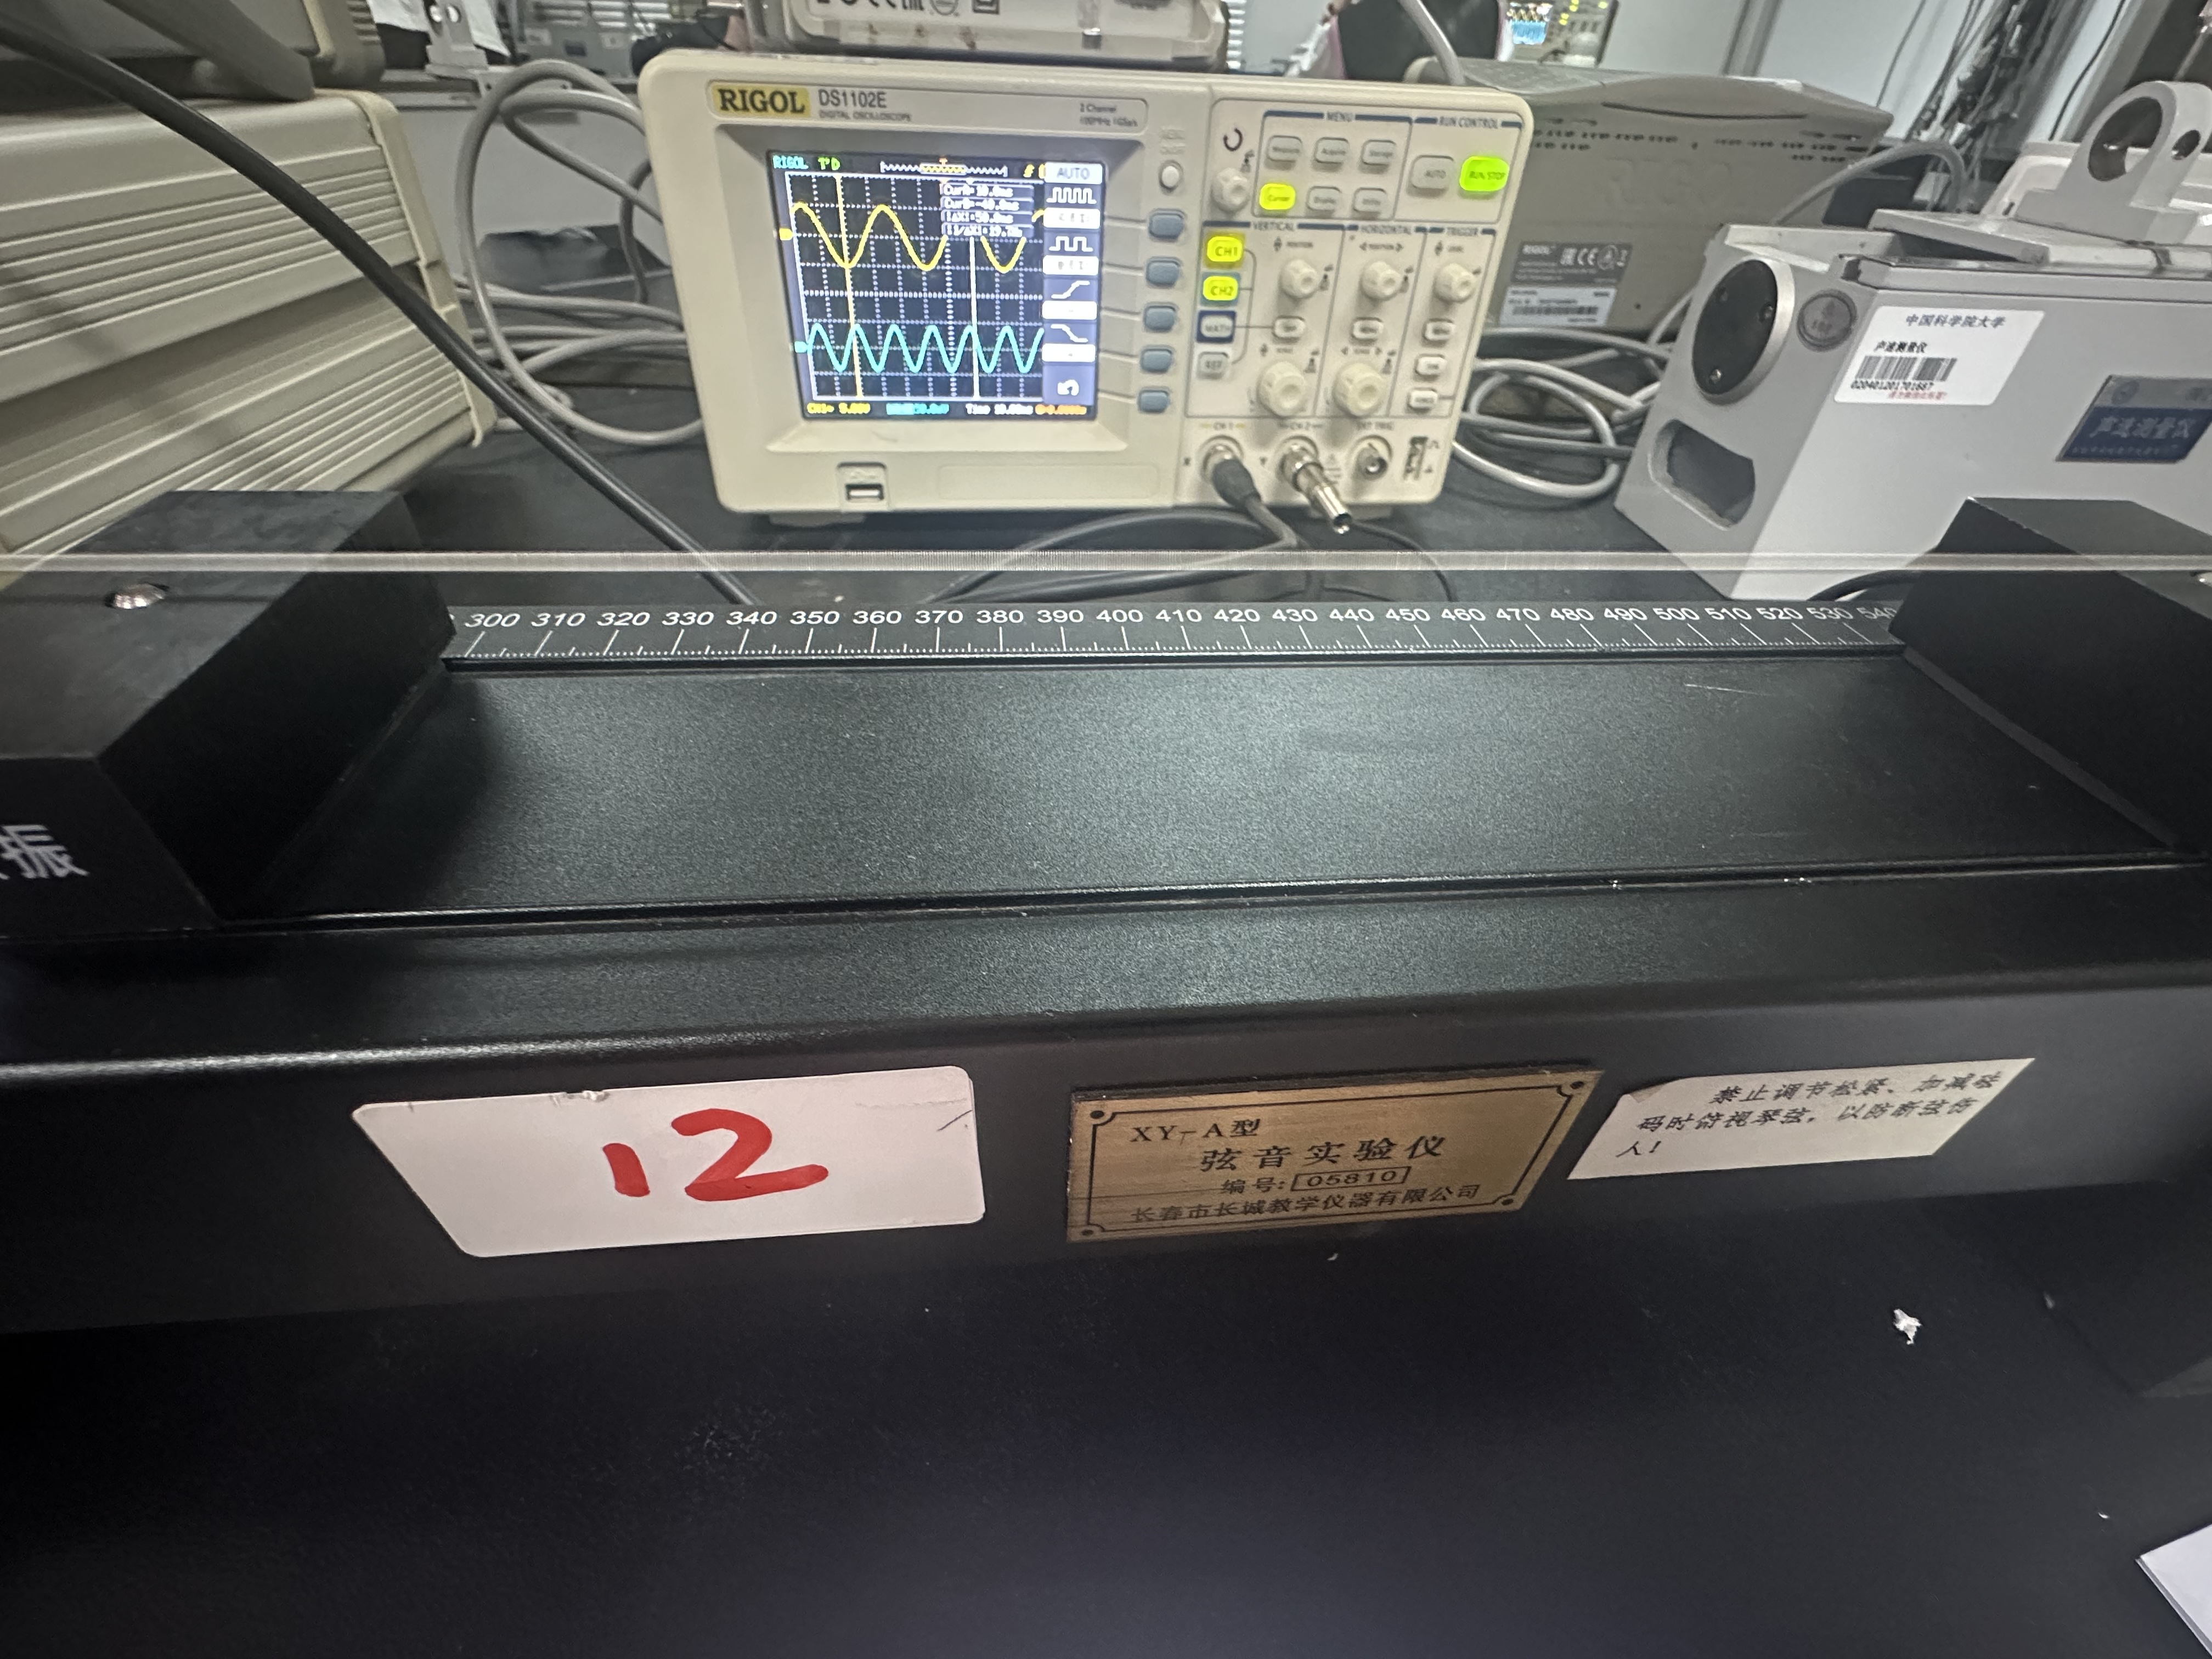
\includegraphics[width=0.8\linewidth]{fig2.jpg} 
    \end{minipage}
    \caption{达到共振状态时的实验记录}
\end{figure}

\subsection{实验数据及处理}
\subsubsection{线密度测试}
\begin{table}[H]
\centering
\begin{tabular}{|c|c|c|c|c|} 
\hline
弦号   &   质量(g)    &   长度(mm)   &  直径(mm)    & 线密度(kg/m)              \\ 
\hline
12 & 0.352 & 61.5 & 1.146 & $5.72 \times 10^{-3}$  \\
\hline
\end{tabular}
\caption{线密度测试}
\end{table}
\subsubsection{波速的测量}
砝码质量$m = 506.10\,\mathrm{g}$, 重力加速度$g = 9.8015 \,\mathrm{m \cdot s^2 / kg}$, 有效长度$L = 500\,\mathrm{mm}$, 频率测量值如下：
\begin{table}[H]
\centering
\begin{tabular}{|c|c|c|c|c|c|c|} 
\hline
砝码位置 & $f_1\ (\mathrm{Hz})$  & $f_2\ (\mathrm{Hz})$  & $f_3\ (\mathrm{Hz})$     & $v_{\text{测量}}= \lambda f \ (\mathrm{m / s})$    & 张力$T \, (\mathrm{N})$    & $v_{\text{理论}} = \sqrt{T / \mu}\ (\mathrm{m / s})$  \\
\hline
2    & 33.63 & 67.63 & 101.69 & 33.78 & 4.961 & 29.44  \\ 
\hline
3    & 43.75 & 87.25 & 130.93 & 43.67 & 7.441 & 36.06  \\ 
\hline
4    & 46.43 & 92.92 & 139.54 & 46.47 & 9.921 & 41.63  \\
\hline
\end{tabular}
\caption{波速的测量}
\end{table}
这部分的误差较大, 可能是由于线密度测量不够准确, 或者是弦线在共振时加力杠杆难以保持水平导致的
\subsubsection{频率与有效长度的关系}
\begin{table}[H]
\centering
\begin{tabular}{|c|c|c|c|c|c|} 
\hline
$L\ (\mathrm{mm})$  & 640 & 480 & 320 & 240 & 160   \\ 
\hline
$f_1\ (\mathrm{Hz})$ & 31.61 & 38.03 & 57.05 & 75.43 & 115.64  \\
\hline
\end{tabular}
\caption{频率与有效长度的关系}
\end{table}
由
\begin{equation}
    \log\lambda = \frac{1}{2}\log T - \frac{1}{2}\log\mu - \log f\lambda = \frac{2L}{n} = 2L
\end{equation}

可知
\begin{equation}
    \log{2L} = \frac{1}{2}\log T - \frac{1}{2}\log\mu - \log f
\end{equation}
从而我们绘制$\log(2L) \sim \log f$的图像, 并用最小二乘法拟合得到斜率为$-1.05$, 与理论值$-1$较为接近
\begin{figure}[H]
    \centering
    
\includegraphics[width=0.8\textwidth]{plot1.pdf}
    \caption{频率与有效长度的关系} 
\end{figure}

\subsubsection{频率与张力的关系}

\begin{table}[H]
\centering
\begin{tabular}{|c|c|c|c|c|c|} 
\hline
砝码位置 & 1     & 2     & 3     & 4     & 5      \\ 
\hline
$T\ (\mathrm{N})$  & 2.48  & 4.96  & 7.44  & 9.92  & 12.40  \\ 
\hline
$f_1 \ (\mathrm{Hz})$ & 32.71 & 45.72 & 53.49 & 56.89 & 64.37  \\
\hline
\end{tabular}
\caption{频率与张力的关系}
\end{table}

绘制$\log(f_1) \sim \log(T)$的图像, 并用最小二乘法拟合得到斜率为$0.41$

\begin{figure}[H]
    \centering
    
\includegraphics[width=0.8\textwidth]{plot2.pdf}
    \caption{频率与张力的关系}
\end{figure}

可以发现实际拟合斜率和理论值$0.5$有一定误差, 这可能是弦线在共振时加力杠杆难以保持水平导致的

\subsubsection{频率和线密度的关系}
\begin{table}[H]
\centering
\begin{tabular}{|c|c|c|c|c|c|} 
\hline
弦号 & 7       & 2       & 6       & 10      & 11       \\ 
\hline
直径 (mm) & 0.811   & 0.508   & 0.549   & 0.899   & 0.870    \\ 
\hline
线密度$\mu$ (Kg/m) & $3.50 \times 10^{-3}$ & $1.53 \times 10^{-3}$ & $2.15 \times 10^{-3}$ & $3.80 \times 10^{-3}$ & $3.68 \times 10^{-3}$ \\ 
\hline
$f_1 \ (\mathrm{Hz})$ & 32.75   & 43.89   & 43.04   & 33.71   & 33.35    \\
\hline
\end{tabular}
\caption{频率和线密度的关系}
\end{table}

绘制$\log(f_1) \sim \log(\mu)$的图像, 并用最小二乘法拟合得到斜率为$-0.35$

\begin{figure}[H]
    \centering
    
\includegraphics[width=0.8\textwidth]{plot3.pdf}
    \caption{频率和线密度的关系}
\end{figure}

可以发现实际拟合斜率和理论值$-0.5$的误差较大, 且这些数据的线性相关性较差, 造成这一误差的原因可能是每个同学用的砝码质量有一定差距
\subsection{实验总结}
本次实验的关键在于通过示波器接收到的信号大小以及实际观察到的弦的振动幅度以及弦的波形来判断频率, 但是如果仔细观察可能会发现在频率较高、张力较大时, 示波器显示的琴弦震动幅度最大值可能存在两个峰, 这时候可以取两个峰的平均值作为频率, 以减小误差.

另外, 在实验中, 由于弦线在共振时加力杠杆难以保持水平, 也会导致实验数据的误差增大, 所以我们也许可以改进实验仪器, 比如说把砝码杠杆的力用一根绳子连接到弦线上, 并在连接段加一个小轮子, 使得砝码杠杆的力可以在弦线上水平并且平稳传递, 从而减小误差.

同时, 该实验对周围环境的细微变化十分敏感. 有时候可能就是手臂压了一下桌子就可能导致示波器显示的波形发生变化, 所以在实验时要尽量保持实验环境的稳定, 同时需要尽可能在短的时间内完成实验, 以减小外界环境的影响.
\subsection{思考题}
\textbf{调节振动源上的振动频率和振幅大小后对弦线振动会产生什么影响？}
\begin{enumerate}
    \item 调节振动源的频率就是改变弦线驱动力的频率, 也就是弦线振动频率改变. 而且当振动源频率达到弦线基频的整数倍时, 弦线会发生共振, 振幅特别大, 且会形成稳定驻波. 
    \item 调节振动源的振幅大小相当于改变驱动力大小, 改变输入的能量多少. 频率一定的情况下, 振动源振幅越大, 弦线振幅也越大, 更利于观察. 
\end{enumerate}

\textbf{如何来确定弦线上的波节点位置？}
\begin{enumerate}
    \item 通过观察弦线振动的波形, 波腹是振动幅度最大的地方, 波节是振动幅度为零的地方, 通过观察弦线振动的波形, 可以确定波节点位置. 
    \item 如果振动幅度很小, 可以根据弦线长度与波长计算波节位置
\end{enumerate}

\textbf{在弦线上出现驻波的条件是什么？在实验中为什么要把弦线的振动调到驻波现在最稳定、最显著的状态？}
\begin{enumerate}
    \item 出现驻波的条件是振动源的频率是弦线基频的整数倍或者弦线的有效长度是半波长的整数倍, 也就是

\begin{equation}
    L = n\frac{\lambda}{2}, \quad n = 1,2,3 \cdots
\end{equation}

    \item 把弦线的振动调到驻波现在最稳定、最显著的状态可以观察到最明显的驻波现象, 使得误差减小, 计算结果更加精确. 
\end{enumerate}

\textbf{在弹奏弦线乐器时, 发出声音的音调与弦线的长度、粗细、松紧程度有什么关系？为什么？}

由公式
\begin{equation}
    f = \frac{1}{\lambda}\sqrt{\frac{T}{\mu}} = \frac{2}{\lambda}\sqrt{\frac{T}{\pi\rho d^{2}}}
\end{equation}

可知
\begin{enumerate}
    \item 弦线的长度越长, 频率越低, 音调越低；
    \item 弦线的粗细越大, 频率越低, 音调越低；
    \item 弦线的松紧程度越大, 频率越高, 音调越高. 
\end{enumerate}

\textbf{若样品弦线与装置上的弦线直径略有差别, 请判断是否需要修正, 如何进行？}

应当需要修正, 计算线密度的公式为
\begin{equation}
    \mu = \rho\pi\frac{d^{2}}{4}
\end{equation}

所以我们可以使用螺旋测微器分别测量样品弦线与装置上弦线的直径, 通过公式和样本弦线的直径、线密度算出弦线体密度$\rho$, 之后将弦线体密度$\rho$与装置上弦线直径$d$代入公式, 计算得出装置弦线的线密度. 

另外需要注意测量时样品与装置上弦线都应当处于紧绷状态

\textbf{对于某一共振频率, 增大或减少频率的调节过程中, 振幅最大的频率位置往往不同, 如何解释这一现象？}
\begin{enumerate}
    \item 仪器本身的问题: 信号发生器的频率输出经常会发生突变, 很难得到一个准确的读数. 
    \item 加力杠杆没法保持水平的问题: 实验过程中加力杠杆难以保持水平, 会因为琴弦的振动而歪斜.
\end{enumerate}
\section{测定介质中的声速}
\subsection{实验目的}
\begin{enumerate}
    \item 利用驻波法测定波长
    \item 利用相位法测定波长
    \item 计算超声波在空气和水中的传播速率. 
\end{enumerate}
\subsection{实验仪器}
\begin{enumerate}
    \item SW-2 型声速测量仪
    \item 信号发生器
    \item 双踪示波器、水槽
\end{enumerate}
\subsection{实验原理}
\subsubsection{利用驻波法测声速}
\begin{enumerate}
    \item 信号发生器输出频率为$f$的信号给超声发射换能器, 发射换能器将电压信号转成超声波并发射. 接收换能器接收超声波并转换成电压信号给示波器. 
    \item 由声波传输理论可知, 如果接收面和发生面严格平行, 即入射波在接收面上垂直反射, 入射波和反射波相互干涉形成驻波. 此时, 两换能器之间的距离恰好等于其声波半波长的整数倍. 在声驻波中, 波腹处声压最小, 波节处声压最大. 接收换能器的反射界面处为波节, 声压效果最大. 所以, 可以从接收换能器端面声压的变化来判断超声波是否形成驻波. 
    \item 转动鼓轮, 改变两只换能器间的距离, 在一系列特定的距离上, 将会出现稳定的驻波, 记录下出现最大电压数值时标尺上的刻度, 相邻两次最大值对应的刻度值之差即为半波长. 
    \item 声波的频率$f$是一个已知的确定的数值, 测出波长后, 可以用$v = \lambda f$来计算超声波的传播速度. 
\end{enumerate}

\subsubsection{利用相位法测定声速}
\begin{enumerate}
    \item 将发射波和接收波同时输入示波器, 并且以 $X-Y$ 模式显示, 两波的频率相同, 相位不同. 当接收点和发射点的距离变化等于一个波长时, 相位差正好是$2\pi$. 
    \item 实验时, 通过改变发射器和接收器之间的距离, 观察相位的变化, 当相位改变$\pi$, 相应距离的改变量即为半波长, 又声波的频率$f$已知, 根据$v = \lambda f$可求出波速. 
\end{enumerate}
\subsection{实验内容}
这里里空气中的情况为例, 水中需要注意设置超声波频率为$f = 1.7 \ \mathrm{MHz}$
\subsubsection{利用驻波法测声速}
\begin{enumerate}
    \item 按照演示组装试验装置, 调节信号发生器输出波的频率为$f = 40\ \mathrm{kHz}$, 调节示波器的模式为$Y - T$模式；
    \item 转动鼓轮调节换能器位置, 示波器电压最大时记录刻度值, 记录连续的十个数据. 
    \item 使用逐差法计算波长$\lambda$, 利用$v = \lambda f$, 计算$v$并与理论值比较. 
\end{enumerate}

\subsubsection{利用相位法测定声速}
\begin{enumerate}
    \item 按照演示组装试验装置, 调节信号发生器输出波的频率为$f = 40\ \mathrm{kHz}$, 调节示波器的模式为$X - Y$模式；
    \item 转动鼓轮调节发射器与接收器间距离, 当相位改变$\pi$时对应距离改变为半波长. 当相位差为$\pi$的整数倍时李萨如图形为直线, 此时可以记录对应的位置, 一共记录十个数据
    \item 使用逐差法计算波长$\lambda$, 利用$v = \lambda f$, 计算$v$并与理论值比较. 
\end{enumerate}

\begin{figure}[H] 
    \centering
    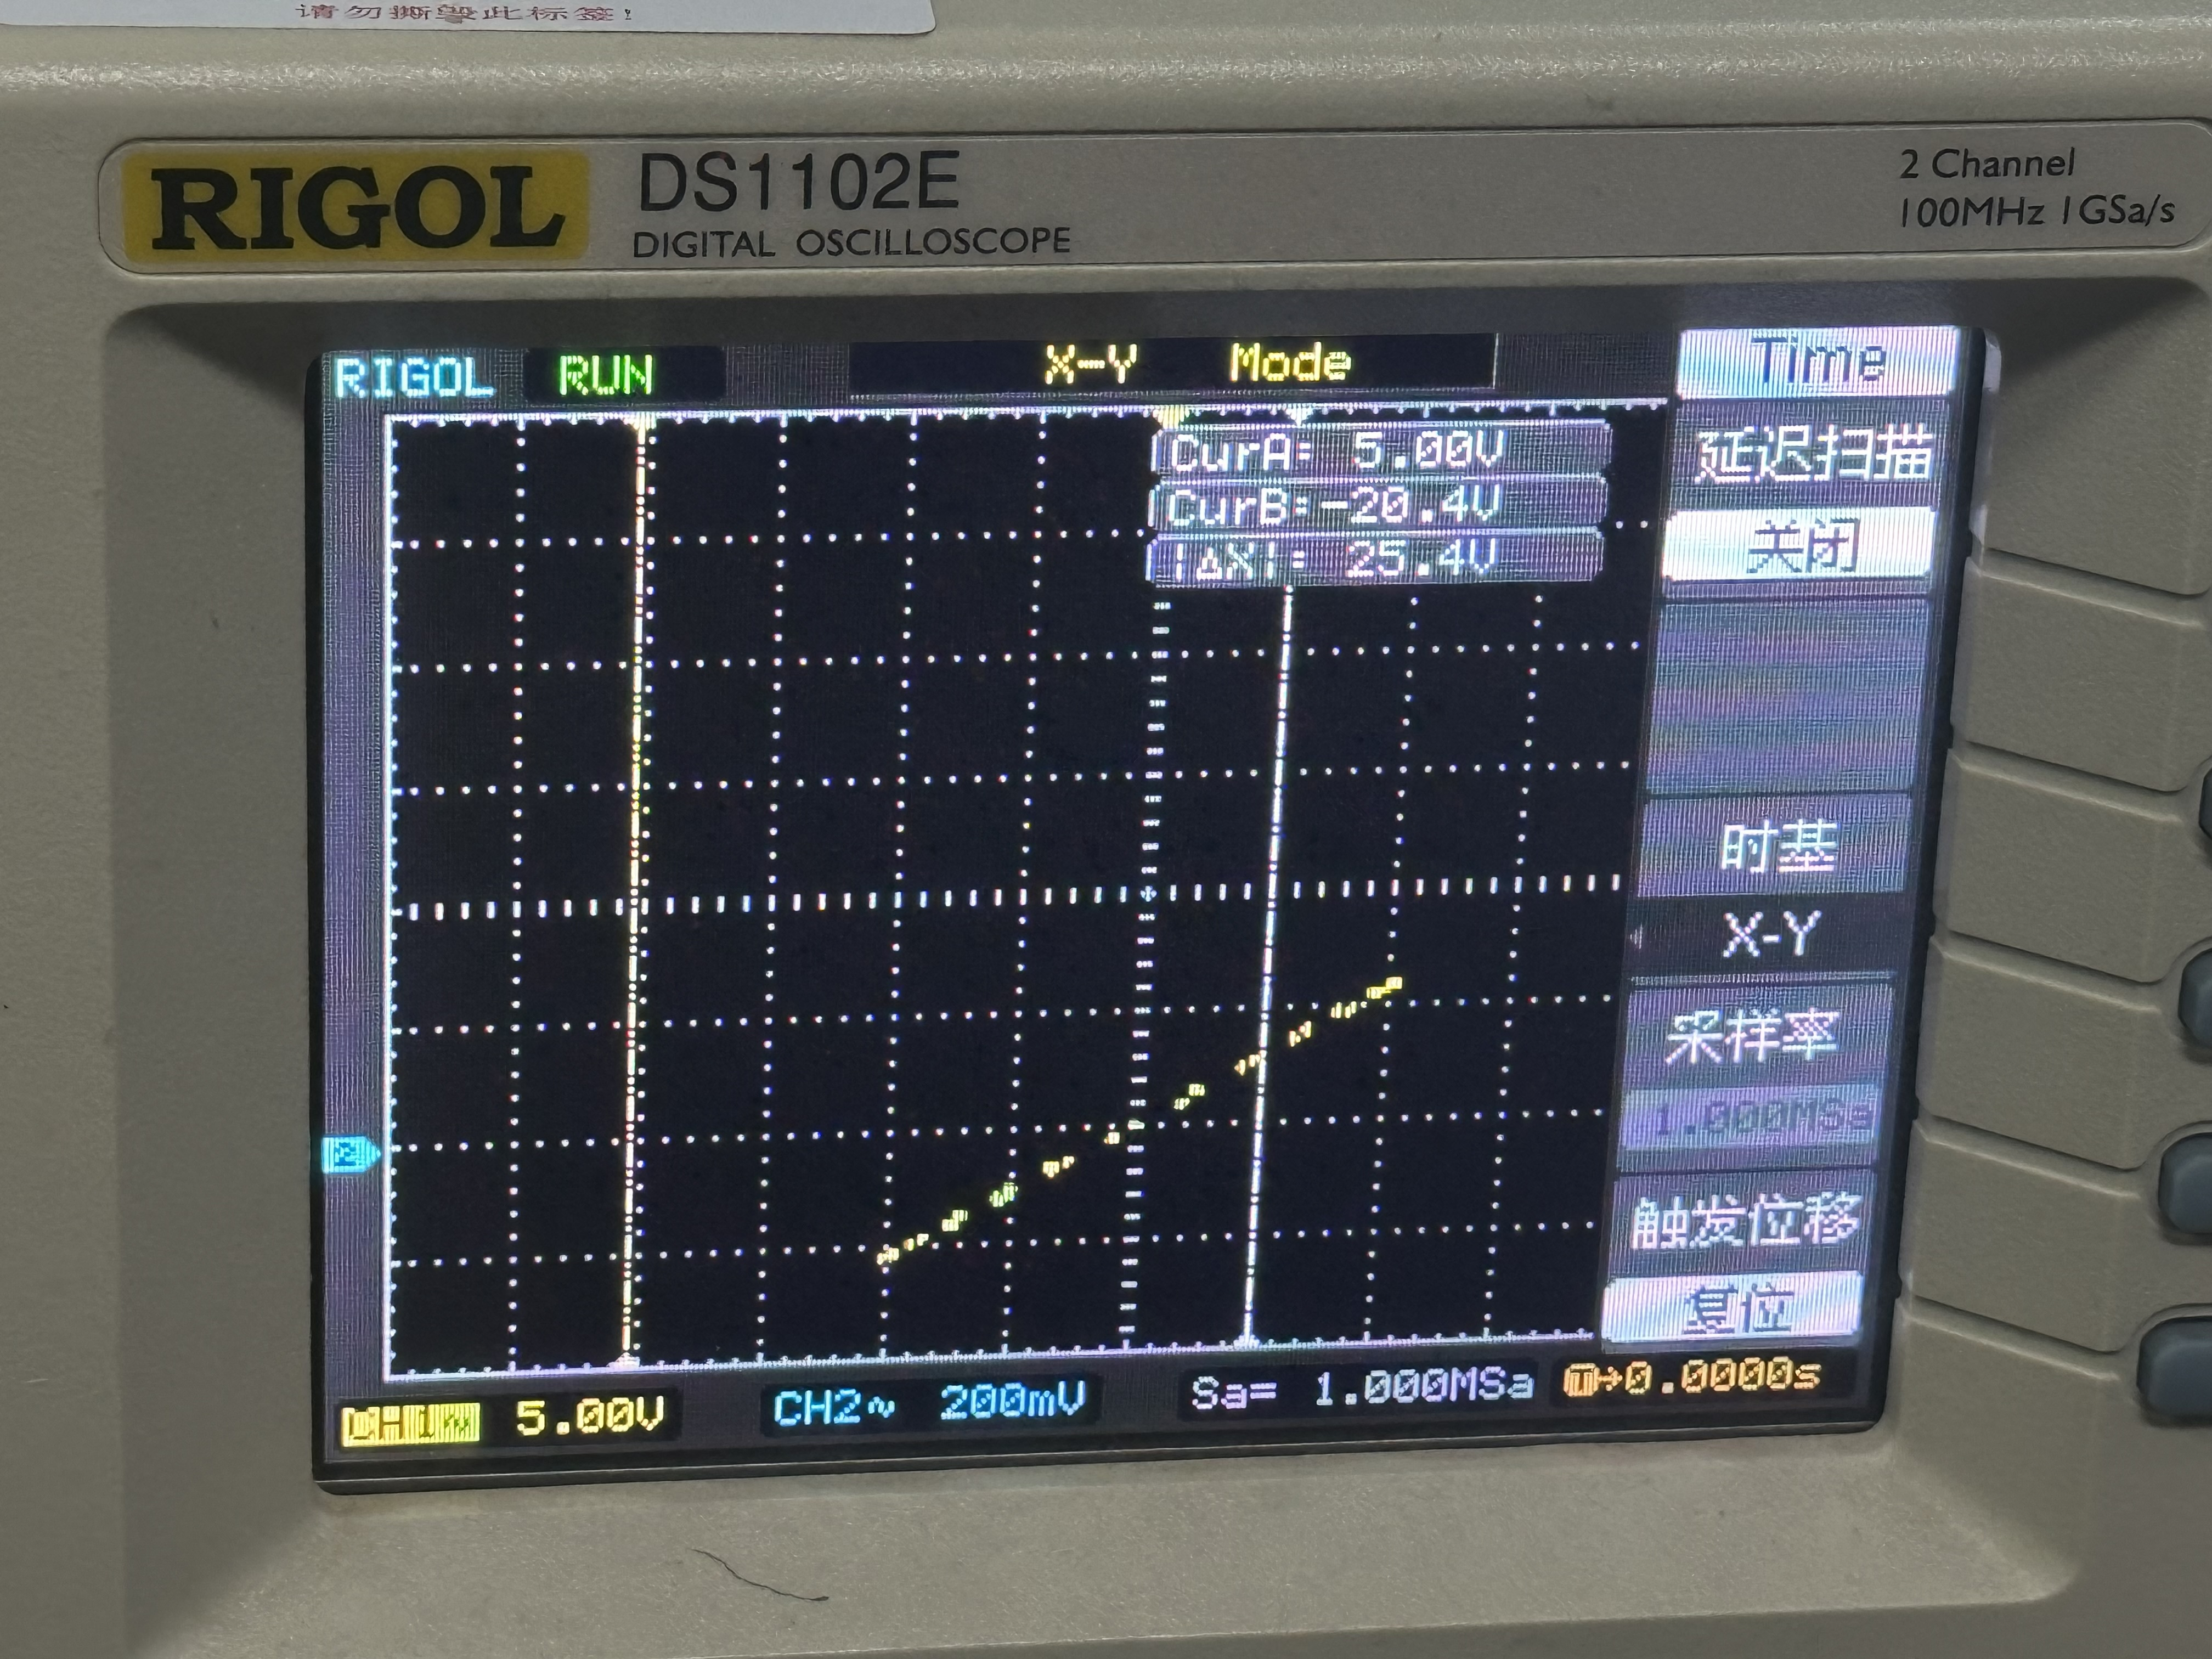
\includegraphics[width=0.6\textwidth]{fig3.jpg}
    \caption{位相法测量声速实验记录}
\end{figure}

\subsection{实验数据及处理}
\subsubsection{空气中超声波波速的测试}
实验参数: $f = 40\  \mathrm{KHz},\  \text{室温} t = 25.9℃$, $V_\text{理论值} = 346.80 \mathrm{m/s}$
\begin{table}[H]
\centering
\begin{tabular}{|c|c|c|c|c|c|c|} 
\hline
$i$  & 驻波法$L_i$ (mm)    & $L_{i + 5} - L_i$ (mm) & $\lambda_i$ (mm) &位相法$L_i$ (mm)  & $L_{i + 5} - L_i$ (mm) & $\lambda_i$ (mm)  \\ 
\hline
1   & 39.698 & 22.114 & 8.846 & 41.483 & 21.568 & 8.627  \\ 
\hline
2   & 43.932 & 22.366 & 8.946 & 45.768 & 21.730 & 8.692  \\ 
\hline
3   & 48.294 & 22.471 & 8.988 & 50.031 & 21.969 & 8.788  \\ 
\hline
4   & 52.750 & 22.555 & 9.022 & 54.228 & 22.324 & 8.930  \\ 
\hline
5   & 57.388 & 22.160 & 8.864 & 58.622 & 22.241 & 8.896  \\ 
\hline
6   & 61.812 &        &       & 63.051 &        &        \\ 
\hline
7   & 66.298 &        &       & 67.498 &        &        \\ 
\hline
8   & 70.765 &        &       & 72.000 &        &        \\ 
\hline
9   & 75.305 &        &       & 76.552 &        &        \\ 
\hline
10  & 79.548 &        &       & 80.863 &        &        \\ 
\hline
平均值 &        & 22.333 & 8.933 &        & 21.966 & 8.787  \\
\hline
\end{tabular}
\caption{空气中超声波波速的测试}
\end{table}

对于驻波法, 计算得实际声速为 $v = \bar{\lambda_i} f = 357.33 \ \mathrm{m/s}$, 相对误差为$E_r = 3.04 \%$

对于相位法, 计算得实际声速为 $v = \bar{\lambda_i} f = 351.46 \ \mathrm{m/s}$, 相对误差为$E_r = 1.34 \%$

\subsubsection{水中超声波波速的测试}

实验参数: $f = 1.7\  \mathrm{MHz},\  \text{室温} t = 25.9℃$; 这里采取\textbf{相位法}进行测量
\begin{table}[H]
\centering
\begin{tabular}{|c|c|c|c|} 
\hline
$i$  & 刻度值$L_i$ (mm)  & $L_{i + 5} - L_i$ (mm) & $\lambda_i$ (mm) \\ 
\hline
1   & 39.981 & 2.197 & 0.879  \\ 
\hline
2   & 40.491 & 2.108 & 0.843  \\ 
\hline
3   & 40.855 & 2.198 & 0.879  \\ 
\hline
4   & 41.332 & 2.193 & 0.877  \\ 
\hline
5   & 41.713 & 2.199 & 0.880  \\ 
\hline
6   & 42.178 &       &        \\ 
\hline
7   & 42.599 &       &        \\ 
\hline
8   & 43.053 &       &        \\ 
\hline
9   & 43.525 &       &        \\ 
\hline
10  & 43.912 &       &        \\ 
\hline
平均值 &        & 2.179 & 0.872  \\
\hline
\end{tabular}
\caption{水中超声波波速的测试(相位法)}
\end{table}

计算得水中声速为 $v = \bar{\lambda_i} f = 1481.72 \ \mathrm{m/s}$
\subsection{实验总结}
这次实验主要利用两个换能器实现电信号和声信号的相互转换，将电信号传入示波器，通过观察示波器上的波形判断此时距离是否满足为半波长的整数倍，一旦驻波条件得到满足就说明二者间的距离达到了波长的整数倍，通过计算两次形成驻波的位置的距离差就可以得到波长的值

在测量空气中的声速时最后的计算结果中相位法相比驻波法更加接近理论值, 这可能是因为在相位法中判断图像是一条斜直线比在驻波法中找出振幅的最大值更加容易直观, 从而带来了更小的度数误差. 正因如此, 我在测量水中声速的实验中选择了使用位相法来测量. 同时, 两种方法测得的声速和理论值还有一定的偏离, 这可能是因为我们没有考虑实验室湿度条件的原因, 湿度条件可能会影响空气的绝热系数, 从而影响声速

\subsection{思考题}
本部分实验没有思考题
\section{附录}
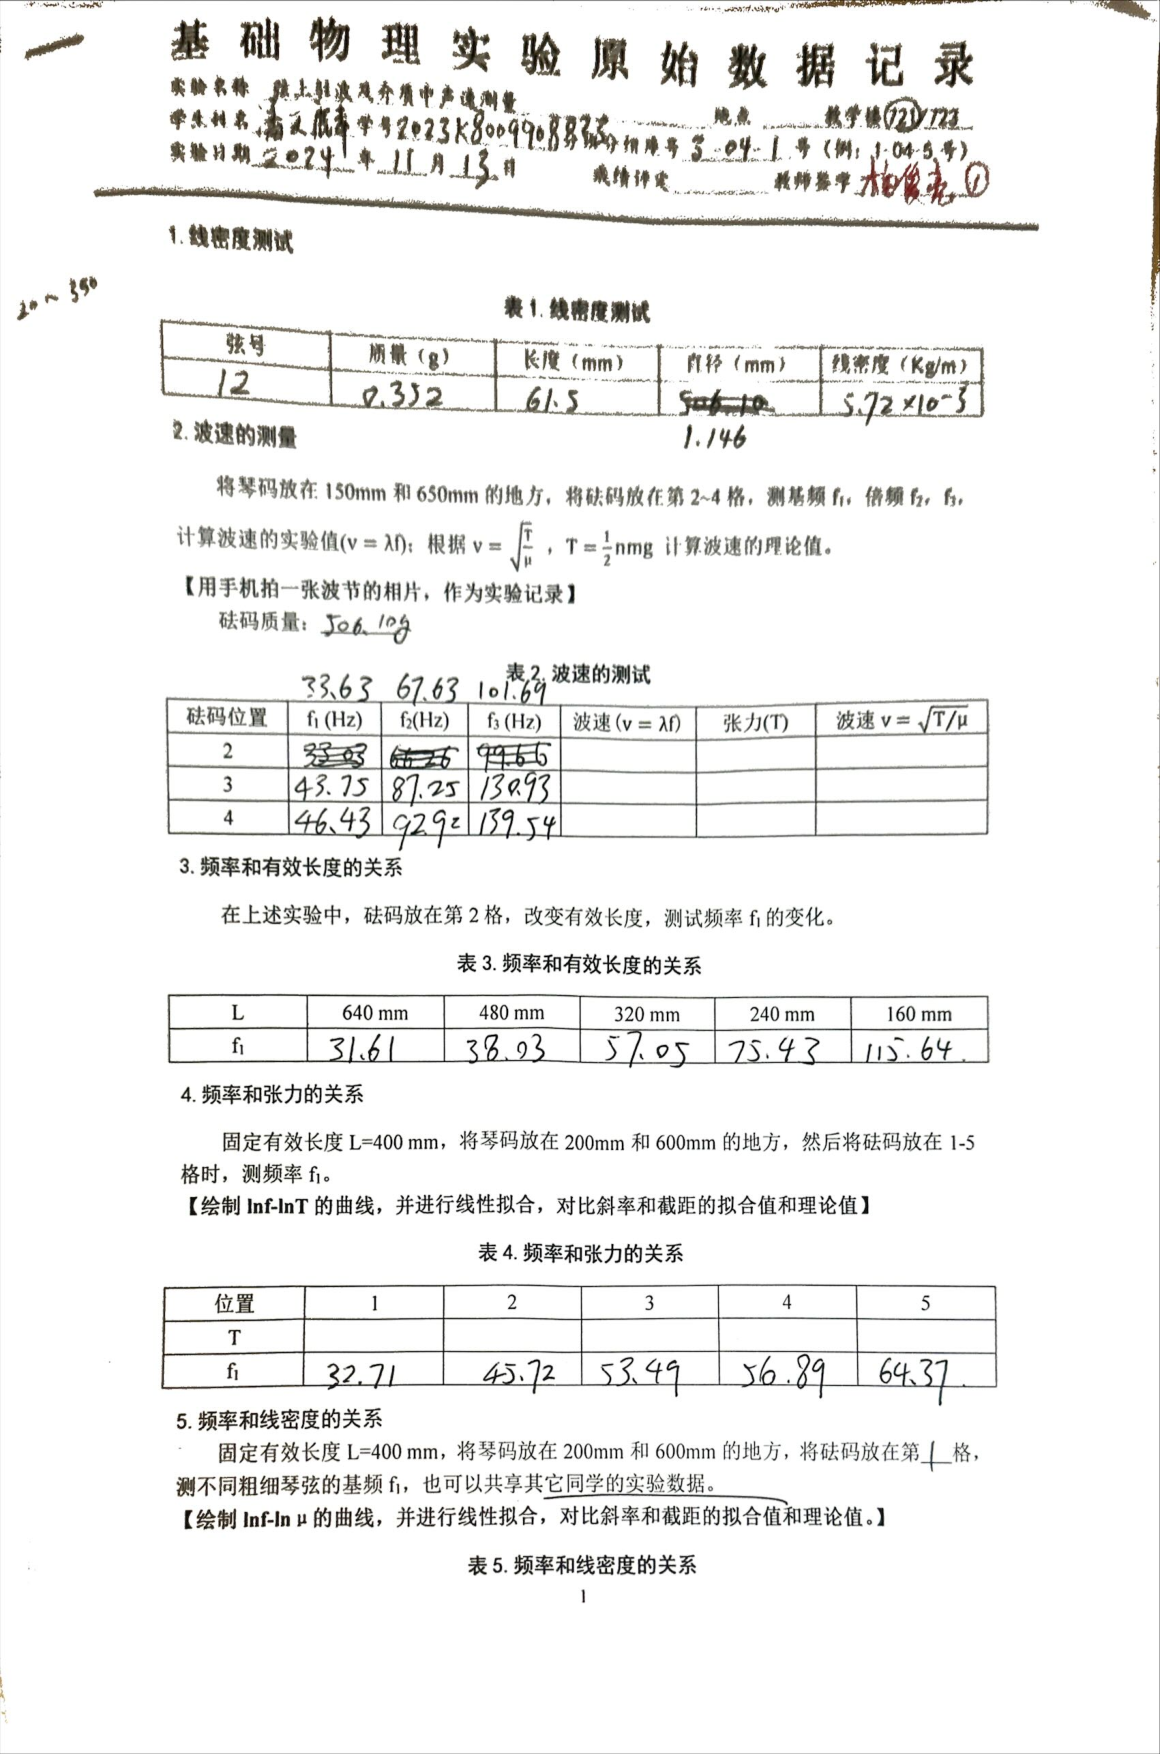
\includepdf[pages=-]{潘天麟-驻波实验-数据.pdf}
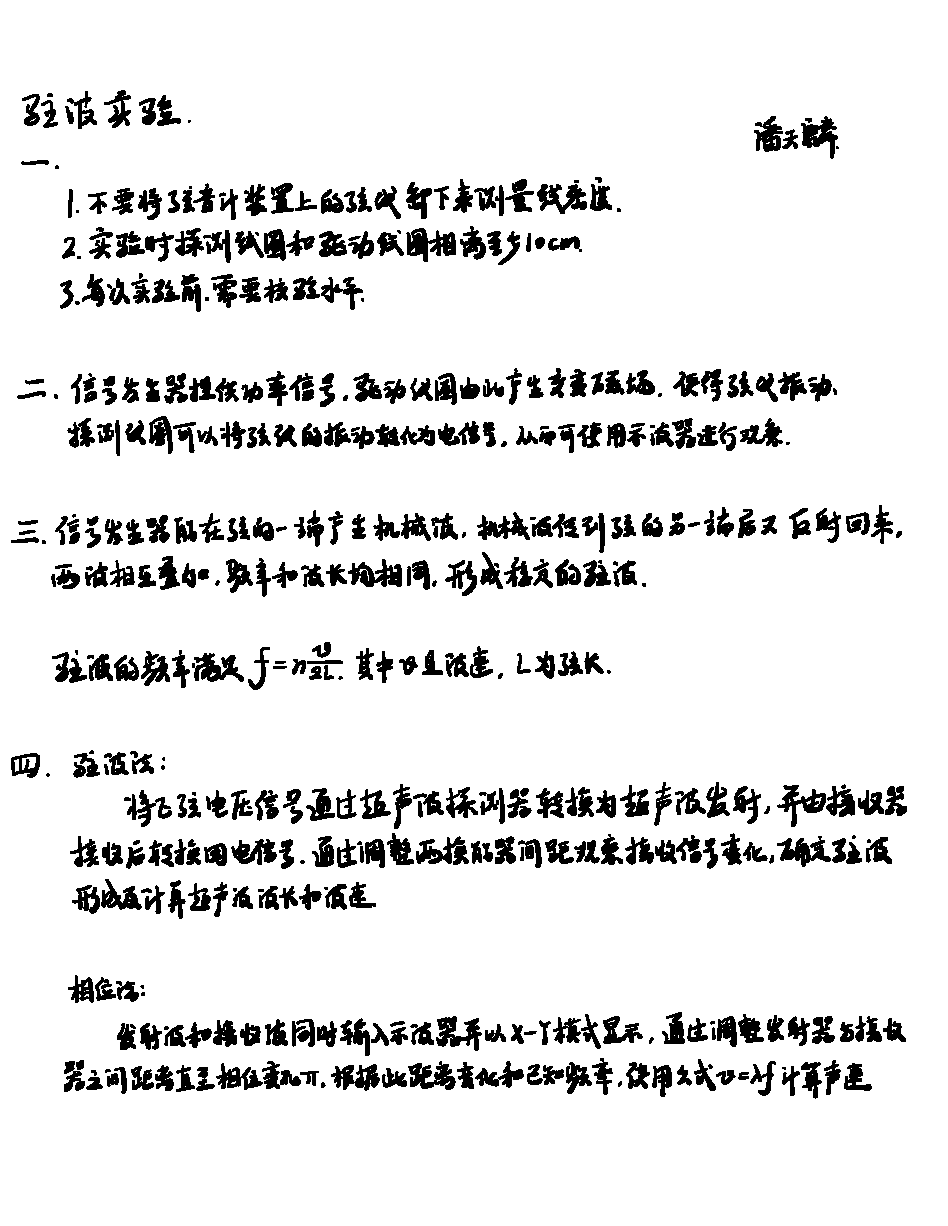
\includepdf[pages=-]{潘天麟-2024-11-13-驻波实验-预习报告.pdf}
\end{document}
